\scanpage{176}
\[
\operatorname{Ext}^p(F,G)
\]
\[
\operatorname{Ext}^{\unsure{p}}(i_!(F),G)\simeq\operatorname{Ext}^p(F,\mathbb{R}i^!(G))
\]
\[
\operatorname{Ext}^*(F,\mathbb{R}i^!(G))\unsure{\Leftarrow|=}E^{pq}=\operatorname{Ext}^p(F,\mathbb{R}^qi^!(\unsure{C|G}))
\]
\margin{\diagram{\begin{tikzcd}[ampersand replacement=\&]Y\arrow[r,hook]\&X\end{tikzcd}}}
\figure{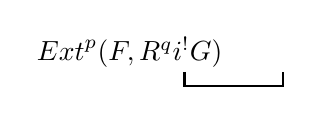
\begin{tikzpicture}[x=1cm,y=1cm]
\node[anchor=west] at (0,0) {$\operatorname{Ext}^p(F,\mathbb{R}^qi^!G)$};
\draw[line width=1pt] (2.0,-0.25)--(2.0,-0.43)--(3.25,-0.43)--(3.25,-0.25);
\end{tikzpicture}}
\[
\operatorname{Ext}^p
\]
\figure{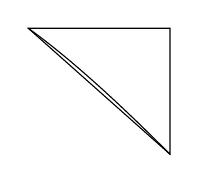
\begin{tikzpicture}[x=1cm,y=1cm]
\draw (0,1.6)--(1.8,1.6)--(1.8,0)--cycle;
\draw (0,1.6) .. controls (0.7,1.1) and (1.5,0.3) .. (1.8,0);
\end{tikzpicture}}
\diagram{$\begin{array}{c@{\quad}c@{\quad}c@{\quad}c@{\quad}c}
\unsure{2d}&\unsure{2d}-1&\unsure{2d}-2&&0\\
\operatorname{Ext}^0,&\operatorname{Ext}^1\ \operatorname{Ext}^2\big/&\operatorname{Ext}^{\unsure{3}}\ \operatorname{Ext}^4\big/&&\big/\operatorname{Ext}^{2d-1},\operatorname{Ext}^{2d}
\end{array}$}
\[
H^p(X,\operatorname{Ext}^q\qquad \deleted{H^{\unsure{n}}}\ H^{\unsure{2d|n}}(X,\operatorname{Ext}^0)+H^{n-1}\operatorname{Ext}^1;
\]
\[
p\leq
\]
\figure{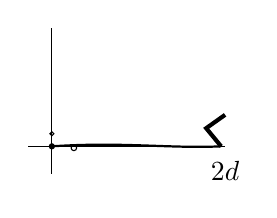
\begin{tikzpicture}[x=1cm,y=1cm]
\draw (-0.3,0)--(2.2,0);\draw (0,-0.35)--(0,1.5);
\fill (0,0) circle(0.04);\draw (0,0.16) circle(0.025);\draw (0.28,-0.02) circle(0.035);
\draw[line width=0.8pt] (0,0)..controls (0.9,0.06) and (1.5,-0.03)..(2.15,0);
\draw[line width=1.5pt] (2.15,0)--(1.96,0.23)--(2.2,0.4);
\node[below] at (2.2,-0.07) {$2d$};
\end{tikzpicture}}
\diagram{$\begin{array}{ccc}
 n\leq2d&n-1\leq2(d-1)&n-3\leq2(d-2)\\
 &\deleted{\unsure{n-1\leq2d-1}}&n-4\leq2(\unsure{2d|d}-2)\\
 &n-2\leq2(d-1)&
\end{array}$}
\[
\deleted{\operatorname{Ext}^*(F,G)\simeq}\qquad\uline{2d-1}
\]
\figure{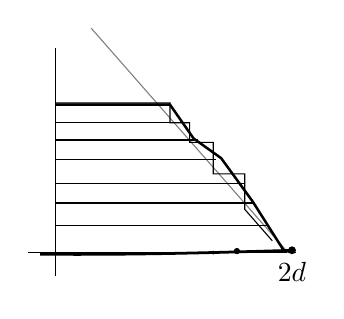
\begin{tikzpicture}[x=1cm,y=1cm]
\draw (-0.35,0)--(3.05,0);\draw (0,-0.3)--(0,2.6);\draw[gray] (0.45,2.85)--(2.95,0);
\draw (0,1.9)--(1.45,1.9)--(1.45,1.65)--(1.7,1.65)--(1.7,1.4)--(2.0,1.4)--(2.0,1.0)--(2.4,1.0)--(2.4,0.55)--(2.75,0.15);
\draw[line width=0.9pt] (0,1.88)--(1.45,1.88)--(1.75,1.45)--(2.1,1.2)--(2.5,0.65)--(2.9,0.02);
\draw (0,1.65)--(1.5,1.65);\draw (0,1.43)--(1.8,1.43);\draw (0,1.18)--(2.04,1.18);\draw (0,0.88)--(2.4,0.88);\draw (0,0.63)--(2.5,0.63);\draw (0,0.35)--(2.7,0.35);
\draw[line width=1pt] (-0.2,-0.02)..controls (1.0,-0.03) and (2.0,0)..(3.02,0.03);
\fill (2.0,0) circle(0.025);\fill (2.3,0.02) circle(0.04);\fill (3.0,0.03) circle(0.05);
\node[below] at (3.0,0) {$2d$};
\end{tikzpicture}}
\[
\mathbb{R}\mathcal{H}om(F,\deleted{\unsure{D}}G)\simeq\mathbb{R}\mathcal{H}om(F\otimes DG,K_X)
\]
\[
\operatorname{Ext}^{\unsure{pq|p+q}}(X;F,\unsure{C|G})\Leftarrow E_2^{pq}=\operatorname{Ext}^{\unsure{pq|p}}(X;\operatorname{Ext}^{-q}(X;G,A_X),A_X)
\]
\[
\operatorname{Ext}^{2d}(X;F,G)
\]
\figure{\begin{tikzpicture}[x=1cm,y=1cm]
\draw (-0.6,1.8)--(2.4,1.8)--(2.4,0)--(0,0);\draw (0,-0.2)--(0,2.2);
\fill (2.4,1.8) circle(0.045);\node[above] at (2.4,1.8) {$2d$};
\end{tikzpicture}}
\figure{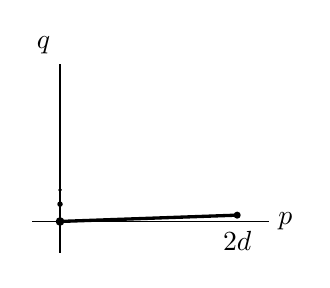
\begin{tikzpicture}[x=1cm,y=1cm]
\draw (-0.35,0)--(2.65,0);\draw (0,-0.4)--(0,2.0);
\draw[line width=1.2pt] (0,0)--(2.25,0.08);\fill (0,0) circle(0.055);\fill (0,0.22) circle(0.035);\fill (0,0.4) circle(0.025);\fill (2.25,0.08) circle(0.045);
\node[above left] at (0,2.0) {$q$};\node[right] at (2.65,0) {$p$};\node[below] at (2.25,0) {$2d$};
\end{tikzpicture}}
\[
\operatorname{Ext}^*(X;F,A_X)\Leftarrow H^p(X,\operatorname{Ext}^q(F,A_X))\qquad 2(d
\]
\[
H^{\unsure{2d|pd}}(X,
\]
\figure{\begin{tikzpicture}[x=1cm,y=1cm]
\draw (0,0)--(3,0);\fill (0,0) ellipse(0.035 and 0.08);\draw (3,-0.04)--(3,0.08);\node[above] at (3,0.08) {$2d$};
\end{tikzpicture}}
\margin{175}
